\documentclass[letterpaper]{article}
\usepackage[utf8]{inputenc}
\usepackage[T1]{fontenc}
\usepackage[activeacute,spanish]{babel}
\usepackage[vmargin=4cm,tmargin=3cm,hmargin=2cm,letterpaper]{geometry}%
\usepackage{helvet}
\usepackage{amsmath,amsfonts,amssymb}
\usepackage{graphicx}
\usepackage{color}
\usepackage{xcolor}
\usepackage{verbatim}
\usepackage{tabls}
\usepackage{lastpage}
\usepackage{fancyhdr}
\usepackage{url}
\usepackage{listings}
%%%%%%%%%%%%%%%%%%%%%%%%%%%%%%%%%%%%%%%%%%%%%%%%%%%%%%%%%%%%%%%%%%%%%%%%%%%%%%%%%%%%%%%
\usepackage{tikz}
\usepackage{pgf}
\usepackage{pgffor}
\usepgfmodule{plot}
\usepackage{wrapfig}
\usetikzlibrary{arrows,decorations,snakes,backgrounds,fit,calc,through,scopes,positioning,automata,chains,er,fadings,calendar,matrix,mindmap,folding,patterns,petri,plothandlers,plotmarks,shadows,shapes,shapes.arrows,topaths,trees}

\lstset{% general command to set parameter(s)
%   basicstyle=\small,
  % print whole listing small
%   keywordstyle=\color{black}\bfseries\underbar,
  % underlined bold black keywords
%   identifierstyle=,
  % nothing happens
%   commentstyle=\color{white}, % white comments
%   stringstyle=\ttfamily,
  % typewriter type for strings
  showstringspaces=false}
  % no special string spaces

\pagestyle{fancy}
\color{black}
\fancyhead{}
\renewcommand{\headrule}{\hrule\vspace*{0.5mm}\rule{\linewidth}{0.8mm}}
\renewcommand{\familydefault}{\sfdefault}

\graphicspath{{./images/}}
\lhead{
\includegraphics[width=2cm]{logoucr.png}}
\rhead{
\includegraphics[width=3cm]{eie-text-gray-6x3cm.png}}
\chead{UNIVERSIDAD DE COSTA RICA\\FACULTAD DE INGENIERÍA\\ESCUELA DE INGENIERÍA ELÉCTRICA\\\textbf{ESTRUCTURAS ABSTRACTAS DE DATOS Y\\ ALGORITMOS PARA INGENIERÍA}\\IE-0217\\I CICLO 2014\\PROPUESTA DE INVESTIGACIÓN BIBLIOGRÁFICA 2}

\lfoot{}%
\cfoot{}%
%\cfoot{\thepage\ de \pageref{LastPage}}%
\rfoot{}%

%%%%%%%%%%%%%%%%%%%%%%%%%%%%%%%%%%%%%%%%%%%%%%%%%%%%%%%%%%%%%%%%%%%%%%%%%%%%%%%%%%%%%%%%%%%%%%%%%%%%%%%%%%%%%%%
\newcommand{\uic}{blue} %user-input color
%%%%%%%%%%%%%%%%%%%%%%%%%%%%%%%%%%%%%%%%%%%%%%%%%%%%%%%%%%%%%%%%%%%%%%%%%%%%%%%%%%%%%%%%%%%%%%%%%%%%%%%%%%%%%%%%%%
\newcommand{\uim}{\_\_} %user-input marker
%%%%%%%%%%%%%%%%%%%%%%%%%%%%%%%%%%%%%%%%%%%%%%%%%%%%%%%%%%%%%%%%%%%%%%%%%%%%%%%%%%%%%%%%%%%%%%%%%%%%%%%%%%%%%%%%%%
\newcommand{\userinput}[1]{\textcolor{\uic}{\uim#1\uim}}


%%%%%%%%%%%%%%%%%%%%%%%%%%%%%%%%%%%%%%%%%%%%%%%%%%%%%%%%%%%%%%%%%%%%%%%%%%%%%%%%%%%%%%%%%%%%%%%%%%%%%%%%%%%%%%%%%%
\begin{document}\vspace*{2cm}
%%%%%%%%%%%%%%%%%%%%%%%%%%%%%%%%%%%%%%%%%%%%%%%%%%%%%%%%%%%%%%%%%%%%%%%%%%%%%%%%%%%%%%%%%%%%%%%%%%%%%%%%%%%%%%%%%%

%%%%%%%%%%%%%%%%%%%%%%%%%%%%%%%%%%%%%%%%%%%%%%%%%%%%%%%%%%%%%%%%%%%%%%%%%%%%%%%%%%%%%%%%%%%%%%%%%%%%%%%%%%%%%%%%%%
\begin{center}
\Huge
\textbf{Knn algorithm using k-d tree}
\vspace*{1cm}
\end{center}

\noindent
\small\baselineskip=14pt
\textbf{Estudiante:} \textbf{Andrés Sánchez López}\\
\textbf{Carné:} \textbf{B26214}\\

%%%%%%%%%%%%%%%%%%%%%%%%%%%%%%%%%%%%%%%%%%%%%%%%%%%%%%%%%%%%%%%%%%%%%%%%%%%%%%%%%%%%%%%%%%%%%%%%%%%%%%%%%%%%%%%%%%
\section{Introducción}

Cada día se requieren hacer búsquedas cada vez más rápidas y eficientes, esto requiere de la busqueda de algoritmos que utilizen estructuras de datos organizadas (como el k-d tree) que organicen la información de tal manera que se logre hacer más rápidas las busquedas. Y las busquedas muchas veces necesitan encontrar cuáles son los k puntos más cercanos a otro ya que muchos programas y algoritmos requieren este tipo de busqueda en su código.

\begin{figure}[h]
\centering
        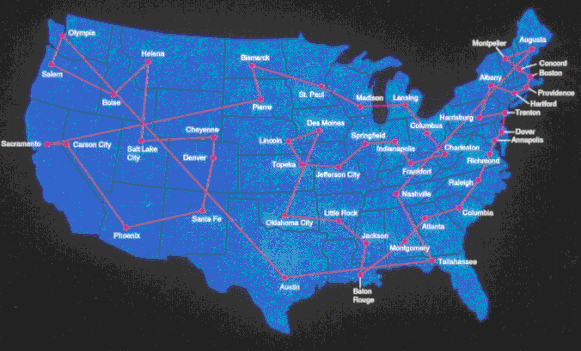
\includegraphics[totalheight=5cm]{map.png}
    \caption{Mapa USA}
    \label{fig:verticalcell}
\end{figure}

Por ejemplo se puede ver en la figura 1 el mapa de USA con distintas locaciones marcadas y se busca la manera de recorrer todas las ciudades de la manera más rápida posible empezando por una ciudad cualquiera(A esto se le llama problema del viajante y tiene muchas aplicaciones), se puede buscar algún algoritmo que busque los vecinos más cercanos y que este algoritmo vaya iterando en cada nodo, buscando el vecino más cercano de cada uno, de tal manera que encuentre cuál es la ruta más rápida posible.  EL algoritmo Knn es precisamente un algoritmo capaz de encontrar los k-vecinos más cercanos a un punto(K nearest neighbors, de ahí el nombre "knn"), por lo tanto se le puede usar para este tipo de problema. Este algoritmo, originalmente, no funciona utilizando un k-d tree pero se puede hacer un algoritmo que haga casi lo mismo que el algoritmo knn pero mediante la utilización de un k-d tree. 
%%%%%%%%%%%%%%%%%%%%%%%%%%%%%%%%%%%%%%%%%%%%%%%%%%%%%%%%%%%%%%%%%%%%%%%%%%%%%%%%%%%%%%%%%%%%%%%%%%%%%%%%%%%%%%%%%%
\section{Objetivos}

\subsection{Objetivo General}

El objetivo general consiste en analizar el funcionamiento y los alcances del algoritmo knn cuando se le programa mediante un k-d tree.\\

\subsection{Objetivos Específicos}

Los objetivos específicos son:\\
\begin{enumerate}
\item Identificar las principales características del algoritmo knn así como algunos de sus usos.
\item Describir el funcionamiento del algoritmo knn utilizando un k-d tree.
\item Entender el algoritmo knn utilizando un k-d tree así como su importancia en la actualidad.
\item Aplicar el conocimiento que se obtenga sobre el algoritmo knn en alguna aplicación.
%\item Comparar el algoritmo knn en su versi\'on original con el que se knn utilizando un k-d tree.
\end{enumerate}

%%%%%%%%%%%%%%%%%%%%%%%%%%%%%%%%%%%%%%%%%%%%%%%%%%%%%%%%%%%%%%%%%%%%%%%%%%%%%%%%%%%%%%%%%%%%%%%%%%%%%%%%%%%%%%%%%%
\section{Metodología}

Lo que se realizará es una investigación bibliográfica sobre una variación del algoritmo knn(utilizando k-d trees) utilizando fuentes primarias, para esto se leerá toda la bibliografía necesaria para poder llegar a entender de la mejor manera como es que funciona esta variación del algoritmo knn y por qué este es necesario, posteriormente se comparará con otros algoritmos utilizados para la misma función, para esto se buscará bibliografía sobre algoritmos que tengan el mismo fin que el knn para poder llegar a entender bien estos algoritmos y poder comprararlos como debe de ser con el knn y ver cuáles son ventajas y desventajas de estos otros algoritmos con respecto al knn, y por lo tanto así determinar de una manera más precisa cuando es que la utilización de esta variación del algoritmo del knn es la mejor opción.\\

También, se buscará alguna implementacion del algoritmo del knn utilizando un k-d tree para demostrar en clase, o se llevará a cabo la implementación de un prototipo demostrativo, para esto se deberá buscar bibliografía que sea de tipo pŕáctica para poder entender ejemplos de problemas o aplicaciones en los que se utilice el algoritmo del knn para resolver ese problema o para lograr la aplicación requerida según sea el caso. Todo lo descrito anteriormente se realizará mediante el siguiente cronograma: \\

\begin{figure}[h]
\centering
        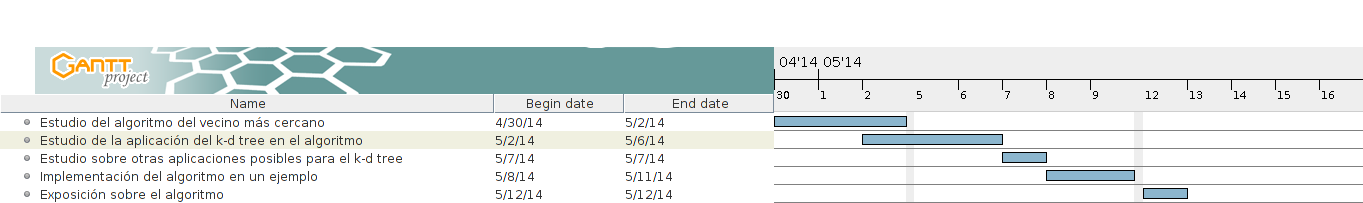
\includegraphics[totalheight=2.8cm]{t.png}
    \caption{Cronograma}
    \label{fig:verticalcell}
\end{figure}

%%%%%%%%%%%%%%%%%%%%%%%%%%%%%%%%%%%%%%%%%%%%%%%%%%%%%%%%%%%%%%%%%%%%%%%%%%%%%%%%%%%%%%%%%%%%%%%%%%%%%%%%%%%%%%%%%%
\section{Referencias}

\begin{enumerate}
\item Hanan Samet. \textit{The design and analysis of special data structures}. Addison Wesley, 1990.
\item Algoritmos y Estructuras de Datos para Búsqueda de Objetos Similares. (n.f). Recuperada 27, Abril, 2014, de:\\ http://www.dcc.uchile.cl/~gnavarro/ps/cita98.pdf.\\
\item How to use a KdTree to search. (n.f). Recuperada 27, Abril, 2014, de:\\
http://pointclouds.org/documentation/tutorials/kdtree\_search.php \\
\item k-Nearest Neighbors. (n.f). Recuperada 27, Abril, 2014, de:\\
http://www.statsoft.com/textbook/k-nearest-neighbors.\\
\end{enumerate}
	
\end{document}

